\section{Separation of Masses}

To speak about static electric and magnetic fields, it is convenient to first introduce the \textbf{Lorentz Force}:
\begin{equation}
    \label{eq:lorentz}
    \vec F = q\left( \vec E + \vec v \times \vec B\right),
\end{equation} which describes the force experienced by a particle of charge $q$ due to an electric ($\vec E$) and/or a magnetic ($\vec B$) field, when moving through them with velocity $\vec v$.

The first term in this force, $q\vec E$, is known as the electric force, which is the force that a particle feels only due to its interaction with an electric field. If the electric field is not time-dependent, it is said to be static. Therefore, the electric force felt by the particle is an \textbf{electrostatic force}. From Newton's second law, which can be written as $\vec F = m\vec a$, we know that a net force on a particle will consitute an acceleration which will be proportional to the magnitude of said force and inversely proportional to the mass of that particle. Considering only static electic fields, the acceleration of a particle of charge $q$ and mass $m$ is:
\begin{equation}
    \label{eq:electrostatic}
    \vec a = \frac{q}{m}\vec E.
\end{equation}

It is therefore possible to study the mass of a particle by the use of electrostatic fields by meausring its acceleration when its charge and the applied electric field is known: 
\begin{equation}
    \label{eq:mass_electrostatic}
    m = \frac{qE}{a},
\end{equation} where now only the magnitudes of the vectors are taken because the acceleration and electrostatic fields are parallel. If this is applied for a radial field, charged particles will feel a centripetal force towards the source of the field, of the form $F_c = m a_c = \frac{mv^2}{r}$, where $r$ is the radius of the trajectory of the particles and $v$ their velocity. In the absence of other forces, the centripetal acceleration will also be the net acceleration, thus $a = a_c = \frac{v^2}{r}$ and therefore, combining this with \autoref{eq:mass_electrostatic}:
\begin{equation}
    \label{eq:centripetal}
    m = \frac{qr}{v^2}E.
\end{equation} 

The resolving power of this technique is only dependent on the precision of the electric field applied, as the charge will remain constant, and radius and velocity are dependent upon the electrostatic field. 

An example of this being used for research is in MARA's electrostatic deflector \cite{saren}, at the University of Jyväskylä. Here, due to the use of two electrodes, the equation is slightly different:
\begin{equation}
    \label{eq:maraE}
    V = \frac{mv^2}{2q}\ln{\left(\frac{R_2}{R_1}\right)} \Rightarrow m = \frac{2qE}{v^2 \ln{\left(\frac{R_2}{R_1}\right)}},
\end{equation} where $R_i$ are the radii of curvature of the outer and inner electrodes. $v$ is only dependent on the energy the recoils are emitted from the target foil at, and q is the charge at which they exit. Thus, only $E$ affects resolution here. \autoref{fig:massresE} shows how mass resolution is affected in MARA by small changes in $E$ differently depending on the original voltage around which the fluctuation happens. As can be seen in the figure, a bigger electrostatic field is less sensitive to fluctuations in terms of mass resolution.

\begin{figure}[H]
    \centering
     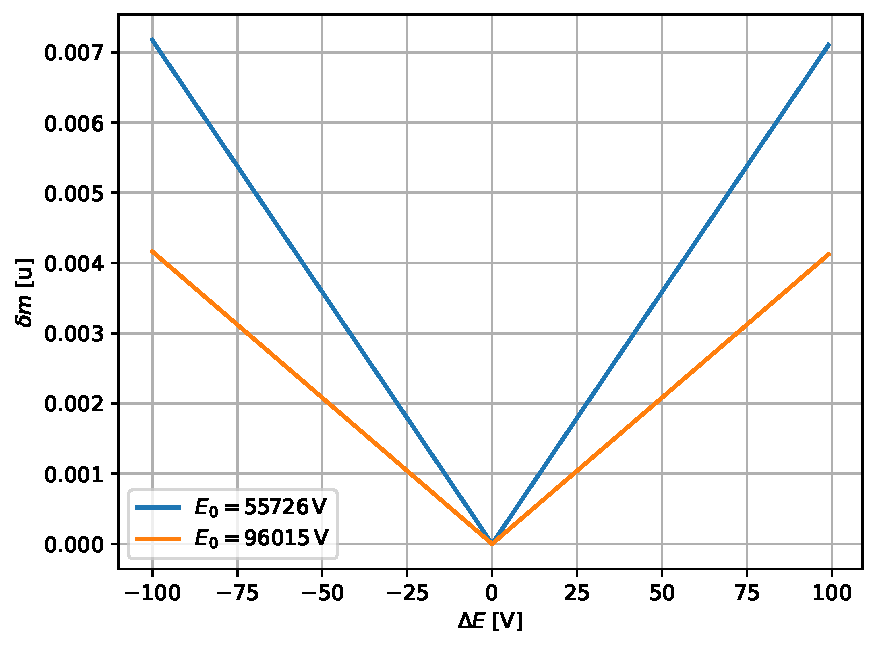
\includegraphics[width=\textwidth]{massresE.pdf}
     \caption{Difference in mass resolution $\delta m$ with respect to the original mass in terms of variations around the optimal field in MARA's electrostatic deflector. Calulated for two alpha particles of different energy and thus different optimal electric field $E_0$.}
     \label{fig:massresE}
 \end{figure}

If, instead of an electrostatic field, a static magnetic field is used, the second term of the Lorentz force (\autoref{eq:lorentz}) comes into play. The \textbf{magnetic force}, $\vec{F} = q(\vec v \times \vec B)$, is the force felt by a charged particle of charge $q$ that traverses a static magnetic field $\vec B$ at velocity $\vec v$. Due to the cross-product, the resulting force is perpendicular both to the magnetic field and the direction of motion. This results in circular paths and therefore a centripetal force. In absence of other forces, this results in:
\begin{align}
    \label{eq:centripetalB}
    F_c &= F_B, \\
    \frac{mv^2}{r} &= qvB, \\
    m &= \frac{qr}{v}B.
\end{align}

Similarly to the electrostatic case, the charge, radius and velocity are fixed for a particle coming into the magnetic field. Thus, only the field strength is relevant. In the case of MARA's dipole magnet \cite{saren}, the dipole radius is $\rho_B = 1\unit{m}$. Since the charge state and speed will be fixed, again there will be a linear dependance between mass resolution and $B$. This will be accentuated at lower $B$ values, as the percentage difference will be higher for the same change around the optimal setting, and a similar shape to that shown in \autoref{fig:massresE} will be seen.

A different way of measuring the mass of a particle is the \textbf{Time of Flight} technique. This technique is based on the fact that applying a force on a particle will result on an acceleration which is inversely proportional to that particle's mass. This is a consequence of Newton's second law, $\vec F = m \vec a$. 

When not under any force, a particle's velocity will be simply defined as the distance it is able to traverse in a certain amount of time, $v = \frac{\d x}{\d t}$. Therefore, if one can measure the time it takes for a particle to traverse a distance after having been accelerated, its mass can be determined as follows:

A particle can be accelerated by a known force which will result in a uniform acceleration $a = F/m$ for a time $t_a$. The acceleration is then stopped, leaving the particle at a constant velocity: $v = \frac{F}{m}t_a$. The particle's linear velocity can be measured in the time interval $t_a$ to $t_f$ by the distance $x$ covered by the particle in that time $v = \frac{x}{t_f - t_a}$, thus arriving at:
\begin{equation*}
    \frac{F}{m} t_a  = \frac{x}{t_f-t_a},
\end{equation*}
thus, the mass of the particle can be obtained as: 
\begin{equation}
    \label{eq:tof}
    m = \frac{Ft_a}{x} (t_f-t_a) = \frac{Ft_a}{x} t_f- \frac{Ft_a^2}{x}.
\end{equation}

Since $F$, the applied force, $t_a$, the time at whih